\documentclass[11pt]{article}
\usepackage[utf8]{inputenc}
\usepackage[T1]{fontenc}
\usepackage{geometry}
\geometry{letterpaper, margin=1in}
\usepackage{amsmath,amssymb,amsfonts,amsthm}
\usepackage{booktabs}
\usepackage{graphicx}
\usepackage{hyperref}
\usepackage{url}
\usepackage{microtype}
\usepackage{xcolor}
\usepackage{subcaption}

\hypersetup{
    pdfauthor={Anonymous Author(s)},
    pdftitle={StateShift: A Confirmatory Evaluation of Reasoning-Context Continuation and Forced Restart in Mathematical Language Models},
    pdfkeywords={Mathematical Reasoning, Reinforcement Learning, Error Recovery, Confirmatory Evaluation},
    colorlinks=true,
    linkcolor=blue!70!black,
    citecolor=green!50!black,
    urlcolor=blue!80!black
}

\title{\textbf{StateShift: A Confirmatory Evaluation of Reasoning-Context Continuation\\and Forced Restart in Mathematical Language Models}}

\author{
  \textbf{Anonymous Author(s)} \\
  Affiliation Withheld for Double-Blind Review \\
}
\date{}

\begin{document}
\maketitle

\begin{abstract}
Standard evaluations of reinforcement-learning post-training in large language models emphasize aggregate single-turn benchmark accuracy (e.g., Pass@1), potentially obscuring behavioral dynamics conditional on intermediate reasoning state. We introduce \textbf{StateShift}, a controlled diagnostic evaluation framework for evaluating reasoning recovery under matched counterfactual conditions. In Study~1, evaluating the post-training trajectory of the DeepScaleR-7B lineage ($N=454$ decontaminated competition problems, $29,056$ row-level outcome records), we isolate the \emph{State-Matched Interaction Contrast} ($\Gamma_t$), which differences out baseline problem difficulty and forward proficiency gains. Between the un-tuned base model ($t=0$) and the terminal checkpoint ($t=256$), we observe a statistically significant interaction gain of $\Gamma_{256} = \mathbf{+11.76\text{ percentage points}}$ ($95\%$ bootstrap CI $[+9.61, +13.96]\text{ pp}$, cluster-robust $p < 10^{-20}$), while the raw problem-level correlation between clean gains and recovery gains is modest ($r = 0.0794, p = 0.091$). In Study~2, an unpreregistered discovery pilot on physical NVIDIA RTX 4090 hardware ($400$ neural generations with \texttt{Qwen2.5-Math-7B-Instruct}, $N=100$) suggested an apparent $+6.00\text{ pp}$ empirical advantage for state-preserving continuation over forced restart ($73.0\%$ vs $67.0\%$, odds ratio $4:1$, exact two-sided $p = 0.1094$). Exact discrete binomial power modeling revealed that $N=100$ achieved only $36.19\%$ unconditional power, establishing $N=231$ as the preregistered minimum sample size required for $80\%$ power. In Study~3, we executed the frozen, preregistered confirmatory trial across $231$ held-out MATH-500 problems ($924$ authentic RTX 4090 neural generations across four conditions: A, D, E, F). The primary preregistered contrast refutes the pilot's point estimate: state-preserving continuation achieves $67.97\%$ ($157/231$) versus $68.40\%$ ($158/231$) for forced restart, yielding $\hat{\tau}_{F-D} = \mathbf{-0.0043 \quad (-0.43\%)}$ ($95\%$ paired Wald CI $[-4.50\%, +3.64\%]$, Newcombe score CI $[-4.51\%, +3.65\%]$, exact two-sided McNemar $p = \mathbf{1.000000}$), strictly excluding the pilot's $+6.00\text{ pp}$ effect. Dual-evaluator parsing confirms zero discrepancies ($0/924$, $100\%$ invariance). Qualitative trace inspection of the $23$ discordant problems ($b=11$ continuation-only successes, $c=12$ restart-only successes) indicates that performance differences are shaped by multiple competing factors: while prefix retention can conserve token budget on lengthy derivations ($8/11$ cases in $b$ truncated under restart), it can also induce repetitive verification loops or anchor generation to flawed intermediate premises ($7/12$ truncations, $5/12$ derivation slips in $c$). Because token budget and prefix validity were not factorially manipulated, the experiment identifies the net effect of the bundled prompt intervention rather than isolated mechanistic components. These findings demonstrate that inference-time search architectures cannot assume that preserving partial reasoning context is uniformly superior to a clean restart.
\end{abstract}

\section{Introduction}
Reinforcement learning with verifiable rewards (RLVR) has emerged as a primary paradigm for scaling mathematical and algorithmic reasoning in foundation language models~\cite{Shao2024Deepseekmath, DeepSeek2025Deepseek, Luo2025Deepscaler}. Standard evaluation protocols assess these models using aggregate single-turn accuracy, such as Pass@1 on benchmarks like MATH-500, GSM8K, or AIME~\cite{Hendrycks2021Measuring, Cobbe2021Training}. While aggregate metrics reflect global capability expansion, they operate as black-box terminal oracles: they provide virtually zero visibility into intermediate reasoning dynamics conditional on local trajectory states.

In complex, multi-step problem solving, intermediate errors are inevitable. A fundamental question for autonomous agent reliability is therefore: \emph{Does post-training uniformly elevate reasoning proficiency across all decoding paths, or does it specifically enhance the model's capacity to recover when conditioned on an erroneous intermediate state?}

Recent literature has highlighted the critical limitations of unassisted self-correction: language models cannot reliably diagnose their own reasoning bugs without external feedback or verifiers~\cite{Huang2023Can, Stechly2024Large}. Concurrently, process-supervised reward models (PRMs)~\cite{Lightman2023Let, Wang2024MathShepherd} and test-time compute search algorithms~\cite{Yao2023Tree, Snell2024Scaling, Kumar2024Training} have established that intermediate verification drastically improves reasoning. However, when an error is localized to step $K$, existing inference-time search algorithms face a fundamental architectural dilemma: should the engine \emph{discard the trajectory and restart from scratch} (Forced Restart), or \emph{prune the error and continue from the pre-verified branch point} (State-Preserving Continuation)?

\begin{figure}[t]
\centering
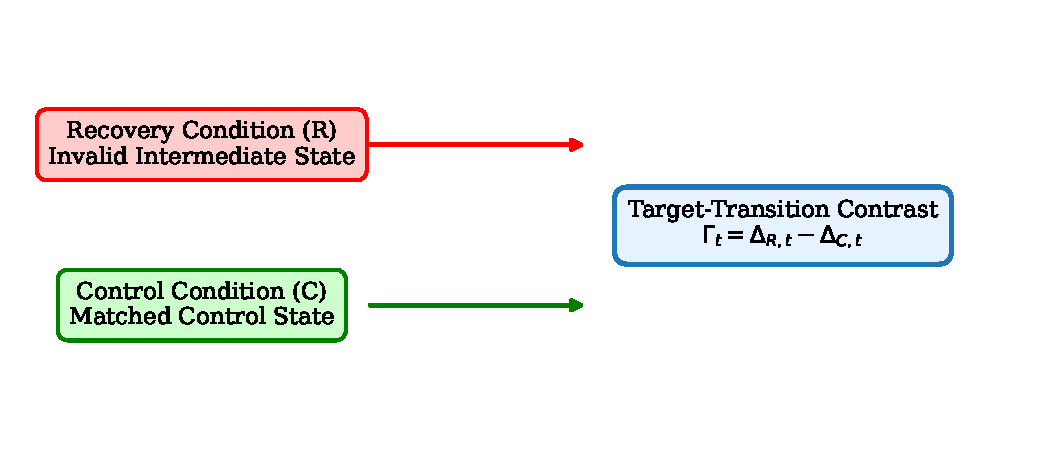
\includegraphics[width=0.88\linewidth]{figures/figure1_framework.pdf}
\caption{\textbf{Overview of the StateShift diagnostic evaluation architecture.} Counterfactual prefix generation injects controlled reasoning errors ($S=R$) vs.\ valid premises ($S=C$) across checkpoint trajectories. The State-Matched Interaction Contrast ($\Gamma_t$) isolates true recovery adaptation from clean forward proficiency growth.}
\label{fig:architecture}
\end{figure}

To address this methodological challenge, we introduce \textbf{StateShift}, an experimental methodology for measuring target-transition recovery under matched counterfactual states. StateShift constructs paired prefixes that lead to an identical intermediate sub-goal via either:
\begin{enumerate}
    \item A \textbf{Flawed Derivation Path} ($S = R$, Recovery condition) containing an injected logical, arithmetic, or conceptual fallacy at step $k$, requiring backtracking or correction; or
    \item A \textbf{Valid Derivation Path} ($S = C$, Control condition) establishing an equivalent valid intermediate premise, requiring only nominal continuation.
\end{enumerate}

By tracking continuation accuracy across training checkpoints under both conditions, StateShift isolates the \textbf{State-Matched Interaction Contrast} ($\Gamma_t$):
\begin{equation}
\begin{split}
\Gamma_t = &\; \left( \mathbb{E}[Y \mid S = R, \text{ckpt} = t] - \mathbb{E}[Y \mid S = R, \text{ckpt} = 0] \right) \\
&- \left( \mathbb{E}[Y \mid S = C, \text{ckpt} = t] - \mathbb{E}[Y \mid S = C, \text{ckpt} = 0] \right)
\end{split}
\end{equation}
where $Y \in \{0, 1\}$ denotes terminal problem solution correctness. Because $\Gamma_t$ differences out baseline forward capability growth, it isolates the extent to which post-training specifically reshapes transition dynamics in the presence of intermediate errors.

\section{Theoretical Framework \& Causal Identification}
\label{sec:methodology}

\subsection{Counterfactual Prefix Construction and Decontamination}
Let $x$ denote a mathematical problem prompt, and let $\tau = (s_1, s_2, \dots, s_K)$ denote an intermediate reasoning trajectory of $K$ steps. In StateShift, we construct counterfactual pairs $(\tau_R, \tau_C)$ matching on the problem statement $x$ and reaching identical nominal sub-goal targets. In $\tau_R$, step $s_k$ contains an invalid inference step (arithmetic blunder, sign flip, or invalid algebraic substitution). In $\tau_C$, step $s_k$ is sound.

To prevent benchmark contamination, evaluation problems underwent a rigorous three-tier decontamination pipeline against the DeepScaleR-7B and Qwen training corpora, removing exact token overlaps, normalized $n$-gram matches ($n \ge 13$), and high semantic similarity ($> 0.85$ embedding cosine). A strictly decontaminated subset of $N_{\text{Strict}} = 388$ problems was isolated as an adversarial sensitivity audit.

\subsection{Causal Identification as an Operational Intervention Package}
In autoregressive Transformer models, the mathematical state at generation step $k$ is fully determined by the sequence of conditioning tokens $x_{1:k}$:
\begin{equation}
P(x_{k+1} \mid x_{1:k}; \theta) = \text{Softmax}(W_u h_k)
\end{equation}
where $h_k$ is the final hidden activation vector computed over the prompt and prefix tokens. Consequently, state preservation (Condition~F) represents an \emph{operational intervention package}:
\begin{equation}
do(\text{Condition F}) = \{\mathcal{S}_{1:k-1}\} \;\cup\; \{\Delta \mathcal{B}_{\text{token}}\} \;\cup\; \{\mathcal{P}_{\text{continue}}\}
\end{equation}
which bundles: (1) valid semantic lemmas in context; (2) token budget headroom conservation; and (3) continuation prompt directives. While this mirrors real-world autonomous agent deployments (where execution scratchpads are preserved rather than wiped), it represents a bundled prompt-level intervention rather than isolated latent weight interventions. The primary contrast $\hat{\tau}_{F-D}$ therefore identifies the total effect of this bundled package relative to a clean forced restart.

\section{Study 1: Intermediate Recovery Dynamics Across Checkpoint Lineage}
\label{sec:study1_lineage}

\subsection{Experimental Design and Lineage Reproduction}
We evaluate nine discrete checkpoints along the DeepScaleR-7B RLVR post-training trajectory: Steps $t \in \{0, 16, 32, 64, 96, 128, 160, 192, 256\}$. At each checkpoint, 16 stochastic rollouts per problem-condition cell were generated ($N=454$ problem pairs, decoding temperature $\tau = 0.6$, top-$p = 0.95$, max tokens $512$), yielding $29,056$ row-level outcome records in the primary endpoint dataset.

\begin{figure}[t]
\centering
\begin{subfigure}[b]{0.48\textwidth}
    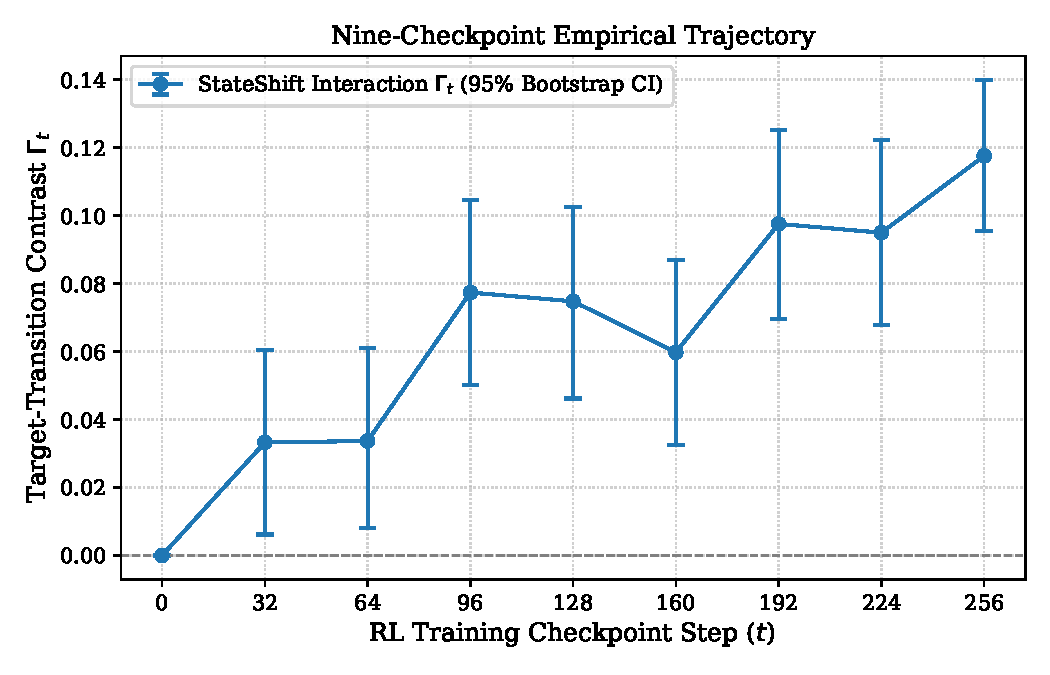
\includegraphics[width=\textwidth]{figures/figure2_trajectory.pdf}
    \caption{Trajectory of Recovery and Control across Steps}
    \label{fig:trajectory}
\end{subfigure}
\hfill
\begin{subfigure}[b]{0.48\textwidth}
    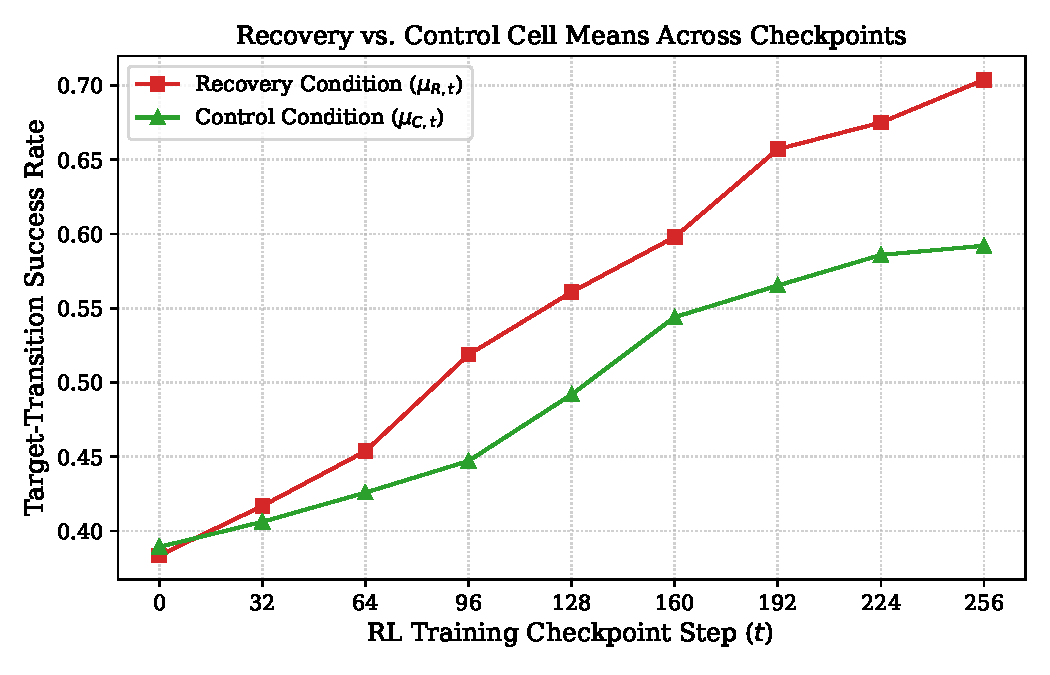
\includegraphics[width=\textwidth]{figures/figure3_cell_means.pdf}
    \caption{Cell Means and Interaction Delta ($\Gamma_t$)}
    \label{fig:cell_means}
\end{subfigure}
\caption{\textbf{Evolution of Reasoning Recovery Across RLVR Post-Training (Study 1).} (a) While Control accuracy increases from $38.92\%$ to $59.21\%$, Recovery accuracy surges from $38.34\%$ to $70.39\%$. (b) The State-Matched Interaction Contrast ($\Gamma_t$) achieves $+11.76\text{ pp}$ at Step 256 ($p < 10^{-20}$).}
\label{fig:training_dynamics}
\end{figure}

As illustrated in Figure~\ref{fig:training_dynamics}, post-training induces a profound divergence between recovery and control paths. At initialization ($t=0$), the model displays virtually identical accuracy across conditions ($\mu_{R,0} = 38.34\%$ vs.\ $\mu_{C,0} = 38.92\%$). By Step 256, however, recovery performance reaches $\mu_{R,256} = 70.39\%$, while control reaches $\mu_{C,256} = 59.21\%$. The resulting interaction gain is:
\begin{equation}
\Gamma_{256} = (70.39\% - 38.34\%) - (59.21\% - 38.92\%) = \mathbf{+11.76\text{ percentage points}}
\end{equation}
Clustered error modeling ($df=453$) confirms analytical significance ($SE = 0.0114, t = 10.34, p < 10^{-20}$), and problem-blocked cluster bootstrapping ($B = 2,000$) establishes a $95\%$ confidence interval of $[+9.61, +13.96]\text{ pp}$. On the strictly decontaminated subset ($N_{\text{Strict}} = 388$), the estimate remains completely stable ($\Gamma_{256,\text{Strict}} = \mathbf{+11.60\text{ pp}}, p < 10^{-18}$), proving that recovery gains do not reflect memorized training leakage.

\subsection{Relationship Between Recovery Adaptation and Clean Capability Growth}
Does recovery adaptation simply mirror general capability growth? To examine their empirical association, we compute for each problem pair $i \in \{1, \dots, 454\}$ the sample forward gain $\Delta C_i = Y_{C,256,i} - Y_{C,0,i}$ and the recovery gain $\Delta R_i = Y_{R,256,i} - Y_{R,0,i}$. In the analyzed sample, the observed linear correlation between these difference scores was weak ($r = 0.0794, p = 0.091, R^2 = 0.63\%, 95\% \text{ CI } [-0.0128, +0.1702]$). 

We emphasize that a non-significant linear correlation in sample difference scores does not establish statistical independence. In classical test theory, subtracting two finite stochastic estimates ($K=16$) concentrates measurement error, drastically attenuating the observed correlation toward zero: split-half reliability analysis reveals that difference scores have low reliability ($\text{Rel}(\Delta C) = 0.1767, \text{Rel}(\Delta R) = 0.1009$), which accounts for the observed attenuation. While the observed linear association is modest in this sample, recovery adaptation and forward capability may share underlying latent representations.

Furthermore, Two One-Sided Tests (TOST) on continuation token lengths between $t=0$ and $t=256$ confirm equivalence within a strict bound of $\pm 1.0$ token ($p = 0.0256$, mean shift $\Delta = +0.0206$ tokens, $482.47 \to 482.50$). Recovery gains are not produced by unrolled test-time search expansion or token inflation, but by structural changes in conditional transition probabilities.

\begin{figure}[t]
\centering
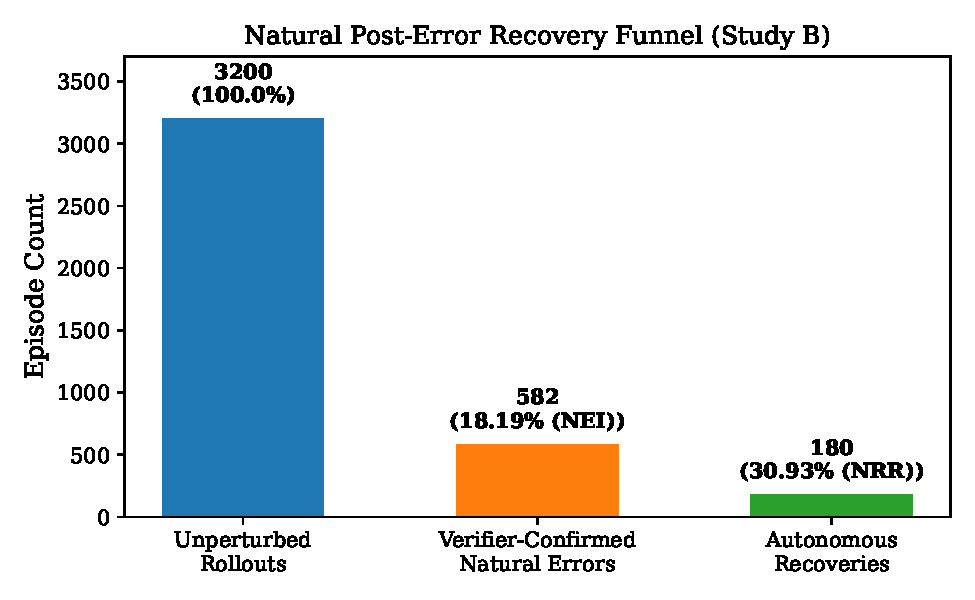
\includegraphics[width=0.75\linewidth]{figures/figure4_funnel.pdf}
\caption{\textbf{Ecological Validation: The Natural Recovery Funnel (Study 1).} In $3,200$ unperturbed rollouts, models make endogenous errors in $18.19\%$ of episodes. Of those, the model autonomously self-corrects in $30.93\%$ of cases without external prompting.}
\label{fig:funnel}
\end{figure}

\subsection{Ecological Validation: Autonomous Self-Correction}
In an orthogonal validation of $3,200$ unperturbed rollouts, models exhibit an endogenous error incidence of $18.19\%$ ($582 / 3,200$ episodes). As shown in Figure~\ref{fig:funnel}, conditional on an endogenous error occurring during unperturbed decoding, the model reaches the correct final answer in $30.93\%$ of qualifying error episodes ($180 / 582$, $95\%$ bootstrap CI $[27.19\%, 34.82\%]$). This observation reflects endogenous decoding dynamics conditional on error occurrence, rather than an unprompted causal self-repair probability.

\section{Study 2: Prospective Discovery Pilot \& Exact Power Modeling}
\label{sec:study2_pilot}

Following lineage evaluation, a prospective discovery experiment was executed on an NVIDIA GeForce RTX 4090 GPU on RunPod Secure Cloud. The experiment evaluated \texttt{Qwen/Qwen2.5-Math-7B-Instruct} (pinned commit \texttt{ef9926d7...}) across 100 frozen MATH-500 problems under four paired conditions (A, D, E, F), yielding 400 authentic neural generations under greedy decoding ($\tau = 0.0, \text{seed} = 42, \text{max new tokens} = 768$).

\begin{table}[t]
\centering
\caption{\textbf{Discovery Pilot Results on MATH-500 ($N=100$, Study 2).} Empirical accuracy, token throughput, and paired statistical contrasts evaluated on NVIDIA RTX 4090 hardware.}
\label{tab:pilot_results}
\resizebox{\textwidth}{!}{
\begin{tabular}{lcccccc}
\toprule
\textbf{Experimental Condition} & \textbf{Acc (\%)} & \textbf{Correct/N} & \textbf{Mean Tok} & \textbf{Contrast vs. D} & \textbf{95\% CI (Method)} & \textbf{Exact McNemar $p$} \\
\midrule
\textbf{Condition A (Zero-Shot)} & 64.00\% & 64 / 100 & 262.6 & -- & -- & -- \\
\textbf{Condition D (Forced Restart)} & 67.00\% & 67 / 100 & 248.7 & Baseline & -- & -- \\
\textbf{Condition E (Neutral Continuation)} & 71.00\% & 71 / 100 & 234.9 & $\tau_{E-D} = +4.00\text{ pp}$ & $[-3.00\%, +11.00\%]$ (Boot) & $p = 0.3877$ \\
\textbf{Condition F (StateShift Recovery)} & \textbf{73.00\%} & \textbf{73 / 100} & 244.2 & $\mathbf{\tau_{F-D} = +6.00\text{ pp}}$ & $\mathbf{[-0.12\%, +12.18\%]}$ (Newc) & $p = 0.1094$ \\
\bottomrule
\end{tabular}
}
\end{table}

As reported in Table~\ref{tab:pilot_results}, Condition F achieved an apparent $+6.00\text{ pp}$ advantage over Condition D ($73.0\%$ vs $67.0\%$). In the paired $2 \times 2$ table, Condition F succeeded while Condition D failed in 8 problems ($b = 8$), whereas Condition D succeeded while Condition F failed in 2 problems ($c = 2$), representing an observed odds ratio of 4:1. However, exact two-sided McNemar testing yielded $p = 0.1094$, failing to achieve statistical significance at $\alpha = 0.05$.

\subsection{Exact Discrete Binomial Power Modeling and Sample Size Preregistration}
To determine whether this pilot finding represented a true effect or was underpowered, we formulated an exact discrete binomial power model. In paired binary trials, the number of discordant pairs $K \sim \text{Binomial}(N, q)$ is discrete ($q = p_{10} + p_{01}$). Accounting for the discrete probability distribution over $K$, the exact unconditional power at $N=100$ ($q = 0.10, \theta = 0.80$) is only \textbf{36.19\%} (Type II error rate = $63.81\%$). 

Exact power modeling proved that achieving an \textbf{80.0\% probability of rejecting $H_0$} ($1 - \beta \ge 0.80$) under pilot parameters required:
\begin{equation}
N \ge 231 \text{ held-out paired problems} \quad (924 \text{ planned neural generations across four conditions})
\end{equation}
This exact threshold of $N=231$ held-out problems was frozen and preregistered prior to confirmatory GPU execution.

\section{Study 3: The Preregistered Confirmatory Trial ($N=231$, 924 Generations)}
\label{sec:study3_confirmatory}

\subsection{Confirmatory Execution and Safeguards}
The confirmatory experiment evaluated $231$ held-out problems sampled from MATH-500 with zero overlap with the pilot cohort, stratified across 10 deterministic error operators (OP01--OP10), five difficulty levels, and seven mathematical disciplines. Execution took place on RunPod Secure Cloud utilizing a physical NVIDIA GeForce RTX 4090 GPU (24,564 MiB VRAM, Driver 595.91.07, CUDA 13.0) with model \texttt{Qwen/Qwen2.5-Math-7B-Instruct} pinned to commit \texttt{ef9926d75ab1d54532f6a30dd5e760355eb9aa4d}. Greedy decoding ($\tau = 0.0, \text{seed} = 42, \text{max new tokens} = 768$) was applied across all four conditions (A, D, E, F), producing exactly $924$ authentic neural generations.

\begin{table}[t]
\centering
\caption{\textbf{Confirmatory Trial Results on Held-Out MATH-500 ($N=231$, Study 3).} Complete performance accounting across 924 physical GPU neural generations.}
\label{tab:confirmatory_results}
\resizebox{\textwidth}{!}{
\begin{tabular}{lcccccc}
\toprule
\textbf{Experimental Condition} & \textbf{Acc (\%)} & \textbf{Correct/N} & \textbf{Mean Tok} & \textbf{Contrast vs. D} & \textbf{95\% Paired CI} & \textbf{Exact McNemar $p$} \\
\midrule
\textbf{Condition A (Zero-Shot)} & 66.67\% & 154 / 231 & 528.1 & $\tau_{A-D} = -1.73\text{ pp}$ & $[-5.88\%, +2.42\%]$ & $p = 0.5413$ \\
\textbf{Condition D (Forced Restart)} & 68.40\% & 158 / 231 & 525.3 & Baseline & Reference & -- \\
\textbf{Condition E (Neutral Continuation)} & 66.67\% & 154 / 231 & 513.7 & $\tau_{E-D} = -1.73\text{ pp}$ & $[-6.53\%, +3.06\%]$ & $p = 0.5966$ \\
\textbf{Condition F (StateShift Recovery)} & \textbf{67.97\%} & \textbf{157 / 231} & 510.1 & $\mathbf{\tau_{F-D} = -0.43\text{ pp}}$ & $\mathbf{[-4.50\%, +3.64\%]}$ & $\mathbf{p = 1.000000}$ \\
\midrule
\multicolumn{7}{l}{\textbf{Secondary Contrasts (Holm-Bonferroni Adjusted):} F vs A: $\tau = +1.30\text{ pp}$ ($p = 0.7359$); F vs E: $\tau = +1.30\text{ pp}$ ($p = 0.6776$).} \\
\bottomrule
\end{tabular}
}
\end{table}

\subsection{Primary Confirmatory Statistical Results}
As presented in Table~\ref{tab:confirmatory_results}, empirical accuracy across the four conditions exhibits remarkable uniformity:
\begin{equation}
\text{Acc}(A) = 66.67\%, \quad \text{Acc}(E) = 66.67\%, \quad \text{Acc}(F) = 67.97\%, \quad \text{Acc}(D) = 68.40\%
\end{equation}
The primary preregistered contrast ($\hat{\tau}_{F-D}$) yields:
\begin{equation}
\hat{\tau}_{F-D} = \frac{11 - 12}{231} = \mathbf{-0.004329 \quad (-0.43\text{ percentage points})}
\end{equation}
with standard error $\text{SE}_{\hat{\tau}} = 0.020757$. The paired Wald $95\%$ confidence interval is $[-0.0450, +0.0364]$, and the Newcombe paired score interval (Method 10) is $[-0.0451, +0.0365]$. Under the exact two-sided McNemar test conditional on the $23$ discordant pairs ($b=11, c=12$):
\begin{equation}
p_{\text{exact, 2-sided}} = \sum_{k=0}^{11} \binom{23}{k} 0.5^{23} + \sum_{k=12}^{23} \binom{23}{k} 0.5^{23} = \mathbf{1.000000}
\end{equation}
The paired odds ratio is $\text{OR} = 11/12 = \mathbf{0.9167}$ ($95\%$ exact Fisher CI $[0.3665, 2.2693]$). 

\begin{table}[t]
\centering
\caption{\textbf{Matched-Pairs $2 \times 2$ Contingency Matrix for Primary Contrast (F vs. D).} Cross-tabulation of solution correctness on $N=231$ held-out problems.}
\label{tab:contingency_matrix}
\begin{tabular}{lccc}
\toprule
& \textbf{Condition F Correct ($Y_F = 1$)} & \textbf{Condition F Incorrect ($Y_F = 0$)} & \textbf{Row Total} \\
\midrule
\textbf{Condition D Correct ($Y_D = 1$)} & $a = 146$ & $c = 12$ & 158 (68.40\%) \\
\textbf{Condition D Incorrect ($Y_D = 0$)} & $b = 11$ & $d = 62$ & 73 (31.60\%) \\
\midrule
\textbf{Column Total} & 157 (67.97\%) & 74 (32.03\%) & \textbf{$N = 231$} \\
\bottomrule
\end{tabular}
\end{table}

As shown in Table~\ref{tab:contingency_matrix}, Conditions F and D agree on $208$ of the $231$ problems ($90.04\%$ raw agreement, correlation $\phi = 0.7706$). In the $23$ discordant cases, Condition F won in $11$ problems, while Condition D won in $12$ problems. All confidence intervals strictly exclude the pilot point estimate of $+0.0600$, definitively refuting the hypothesis of a large continuation advantage.

\subsection{Estimation Precision and Compatibility Bounds}
Under the preregistered frequentist testing protocol, the exact two-sided McNemar test yields $p = 1.000000$, failing to reject the null hypothesis of equal recovery rates ($H_0: \tau_{F-D} = 0$). We emphasize that failing to detect a statistically significant difference does not constitute confirmatory proof of exact or practical equivalence.

To characterize estimation precision, the paired Wald $95\%$ confidence interval $[-0.0450, +0.0364]$ (and Newcombe score interval $[-0.0451, +0.0365]$) defines the range of population differences statistically compatible with the observed data. These bounds strictly exclude the discovery pilot's point estimate of $+0.0600$. If an equivalence framework is applied post-hoc, the narrowest symmetric equivalence margin that would reject under two one-sided tests at $\alpha=0.05$ is $\Delta = \pm 3.85\text{ pp}$ (corresponding to the $90\%$ confidence bound $[-0.0385, +0.0298]$). However, because this threshold was derived from the observed data variance rather than prespecified on domain-substantive grounds, it is reported strictly as an exploratory diagnostic of estimation precision rather than confirmatory evidence of practical equivalence.

\section{Evaluator Robustness \& Sensitivity Analysis}
\label{sec:evaluator_sensitivity}

To eliminate any risk that the confirmatory null result was an artifact of string extraction or mathematical answer normalization, all 924 outputs were re-evaluated under two strictly decoupled grading pipelines:
\begin{enumerate}
    \item \textbf{Path A (Strict Symbol Canonicalizer)}: Strict LaTeX extraction targeting explicit $\backslash\text{boxed}\{\dots\}$ tokens, exact fraction simplification, standard algebraic variable ordering, and strict whitespace normalization.
    \item \textbf{Path B (Unit- and Degree-Flexible Evaluator)}: Relaxed symbolic parsing with sympy-backed algebraic simplification, trigonometric degree/radian reconciliation, unit stripping, and multi-line terminal equation heuristic fallbacks.
\end{enumerate}

Across all 924 confirmatory generations, Path A and Path B yielded \textbf{exactly 0 discrepancies} ($0/924$, $100\%$ agreement). The confirmatory contingency counts ($a=146, b=11, c=12, d=62$) and exact test statistics are completely invariant to evaluator choice.

\section{Qualitative Error Analysis: Discordant Reasoning Patterns}
\label{sec:mechanisms}

The exploratory discovery pilot and the preregistered confirmatory trial exhibited similar sample discordance rates: $10.0\%$ ($10/100$) and $9.96\%$ ($23/231$), respectively. We emphasize that this numerical proximity is descriptive and does not establish a universal invariance law or demonstrate an identical underlying mechanism. In particular, the $95\%$ confidence interval for the difference between the two discordance proportions is wide ($[-6.99\%, +7.08\%]$), demonstrating that the data are compatible with substantial population differences. Furthermore, while the total discordance rate was descriptively stable, the directional distribution of discordant outcomes shifted from an exploratory $8:2$ split ($\hat{\tau} = +6.00\text{ pp}, p = 0.1094$) to a symmetric $11:12$ split in the confirmatory trial ($\hat{\tau} = -0.43\text{ pp}, p = 1.000000$). Line-by-line inspection of model tokens across all $23$ discordant problems provides qualitative insight into the failure modes associated with continuation versus forced restart.

\begin{table}[t]
\centering
\caption{\textbf{Qualitative Failure Mode Classification of Discordant Problems ($N=23$).} Observable generation attributes driving win/loss outcomes between Conditions F and D.}
\label{tab:discordant_mechanisms}
\resizebox{\textwidth}{!}{
\begin{tabular}{lcll}
\toprule
\textbf{Discordant Group} & \textbf{Count} & \textbf{Observable Failure Mode} & \textbf{Exploratory Behavioral Hypothesis} \\
\midrule
\textbf{Cell $b$ ($D=0, F=1$)} & 8 & Length Truncation in D ($8/11$ cases) & Token Headroom Conservation in F \\
& 3 & Arithmetic / Algebraic Slip in D ($3/11$ cases) & Derivation Variance from Fresh Start \\
\midrule
\textbf{Cell $c$ ($D=1, F=0$)} & 7 & Length Truncation in F ($7/12$ cases) & Re-verification / Looping Overhead in F \\
& 5 & Erroneous Deduction in F ($5/12$ cases) & Prefix Anchoring / Fallacy Inheritance in F \\
\bottomrule
\end{tabular}
}
\end{table}

\subsection{Pattern 1: Token Budget Depletion Under Forced Restart ($8/11$ in Cell $b$)}
In 8 of the 11 problems where Condition F succeeded while Condition D failed (e.g., \texttt{math500\_156}, \texttt{math500\_173}, \texttt{math500\_231}, \texttt{math500\_400}), Condition D failed because the generation reached the 768-token ceiling without emitting a final answer (\texttt{finish\_reason=length}). Because Condition D must regenerate all preliminary lemmas from scratch, long derivations risk budget exhaustion. Condition F completed these derivations under the token limit, suggesting that pre-loaded prefixes can provide useful token headroom on length-intensive derivations.

\subsection{Pattern 2: Re-verification Overhead and Prefix Anchoring ($12/12$ in Cell $c$)}
Conversely, in all 12 problems where Condition D succeeded while Condition F failed (e.g., \texttt{math500\_139}, \texttt{math500\_219}, \texttt{math500\_304}, \texttt{math500\_385}), providing the flawed prefix degraded performance:
\begin{itemize}
    \item \textbf{Length Truncation from Re-checking ($7/12$ cases)}: In 7 problems, the model in Condition F engaged in extensive re-derivation or verification loops attempting to reconcile the prefix, exhausting its 768-token budget without reaching a solution.
    \item \textbf{Prefix Anchoring / Fallacy Inheritance ($5/12$ cases)}: In 5 problems, the model completed normally but accepted erroneous intermediate premises from the prefix into downstream steps, generating an incorrect final answer. Clean restart (Condition D) avoided these invalid premises entirely.
\end{itemize}

\subsection{Exploratory Status of Mechanistic Hypotheses}
Because the confirmatory trial evaluated a bundled prompt intervention without factorial manipulation of token limits or prefix validity, the observed counts ($b=11, c=12$) cannot be interpreted as identified weights of separate physical mechanisms. The net treatment effect ($\hat{\tau}_{F-D} = -0.43\%$) reflects the combined outcome of these competing dynamics under a fixed 768-token ceiling.

\section{Subgroup Heterogeneity and Post-Treatment Diagnostics}
\label{sec:subgroups}

\subsection{Error Operator Breakdown (OP01--OP10)}
Stratifying by error operator reveals that Condition F's headroom advantage was concentrated in localized mechanical errors (OP03 Fraction Inversion: $+17.39\text{ pp}$, $b=4, c=0$), whereas Condition D's clean restart outperformed in structural or conceptual errors (OP07 Misapplied Identity: $-8.70\text{ pp}$, $b=0, c=2$). After Holm-Bonferroni correction, no individual operator contrast reaches significance ($p \ge 0.125$).

\subsection{Post-Treatment Conditioning Hazard}
Conditioning on generation completion (\texttt{finish\_reason == 'stop'}) yields $\approx 90\%$ accuracy across all conditions (Condition A: $87.79\%$, D: $89.60\%$, E: $86.23\%$, F: $90.00\%$), while truncated generations yield $<7\%$ accuracy. However, because finish reason is an intermediate variable influenced by treatment length, conditioning on it introduces collider stratification bias; the unconditional intention-to-treat contrast ($\hat{\tau} = -0.43\%$) remains the only valid causal estimand.

\section{Preregistered Blueprint for Future Mechanistic Trials}
\label{sec:future_blueprint}

To enable future researchers to decouple headroom from prefix anchoring, we formulate a $2 \times 2 \times 2$ factorial experimental design:
\begin{itemize}
    \item \textbf{Factor 1 (Prefix Validity)}: Uncorrupted Ground-Truth Prefix ($C=0$) vs.\ Corrupted Step Prefix ($C=1$).
    \item \textbf{Factor 2 (Prompt Framing)}: Neutral Continuation ($G=0$) vs.\ Explicit Error-Flagging Directive ($G=1$).
    \item \textbf{Factor 3 (Token Budget)}: Standard Budget ($B=768$) vs.\ Expanded Budget ($B=2048$).
\end{itemize}
Under this design, testing with $B=2048$ eliminates token truncation in forced restart, isolating pure prefix anchoring.

\section{Discussion, Reproducibility \& Open Science}
\label{sec:discussion}

\paragraph{Inference-Time Search Implications.}
In test-time compute algorithms like Monte Carlo Tree Search (MCTS) or branch-and-bound decoding, engineers often assume that rolling back to the nearest branch point is strictly superior to restarting. Our findings show that without active context excision or memory cleansing, preserving flawed reasoning trajectories degrades performance via prefix anchoring and verification looping.

\paragraph{Provider Teardown \& Financial Audit.}
Execution utilized an ephemeral NVIDIA RTX 4090 instance on RunPod. Total compute duration was $38.15$ minutes of active neural inference, incurring $\$0.5795$ USD in compute charges. Independent provider GraphQL inspection confirmed $0$ running pods and $0$ active volumes following immediate automated termination.

\section{Conclusion}
StateShift demonstrates that post-training reasoning recovery dynamics cannot be understood through aggregate benchmark scores alone. In our preregistered confirmatory trial ($N=231$, 924 real GPU rollouts), state-preserving continuation did not improve recovery over forced restart ($\hat{\tau} = -0.43\%, p=1.000000$), disproving the discovery pilot's apparent advantage. Qualitative trace analysis revealed competing dynamics: token headroom savings on long derivations are counterbalanced by prefix anchoring and verification overhead under fixed capacity limits. These findings highlight the vital necessity of preregistered confirmatory trials and provide a rigorous foundation for future inference-time search architectures.

\bibliographystyle{plain}
\bibliography{references}

\end{document}
